\section{Lecture 24}
\textsc{Find the mean and variance}

\[ E[X]=\int\limits_{0}^{\infty} x \frac{1}{\theta}e^{-\frac{x}{\theta}} d{x}  \text{ IBP} \]
Trick: \textbf{Gamma Function}
\[ \Gamma(\alpha)=\int\limits_{0}^{\infty} x^{\alpha -1}e^{-x} d{x}  \]
where $ \alpha>0 $

\textsc{Properties of the Gamma Function}

(1) if $ \alpha>1 $, then $ \Gamma(\alpha)=(\alpha-1)\Gamma(\alpha-1) $

(2) if $ \alpha $ is an integer $ \ge 1 $,
\[ \Gamma(1)=1 \]
\[ \Gamma(2)=1\Gamma(1)=1 \]
\[ \Gamma(3)=2\Gamma(2)=2 \]
\[ \Gamma(4)=3\Gamma(3)=6 \]
In general,
\[ \Gamma(\alpha)=(\alpha-1)! \]
So, back to our example:
\begin{align*}
    E[X]&=\int\limits_{0}^{\infty} x \frac{1}{\theta}e^{-\frac{x}{\theta}} d{x}\qquad y=\frac{x}{\theta}\implies x=(\theta y) \land \theta dy=dx\\
    &=\int\limits_{0}^{\infty} (\theta y) \frac{1}{\theta} e^{-y}\theta d{y}\\
    &=\theta \int\limits_{0}^{\infty} y^{2-1}e^{-y} d{y}\qquad \Gamma(2)=(2-1)!=1\\
    &=\theta
\end{align*}
\[ E[X]=\theta=\frac{1}{\lambda} \]
Why?
If $ \lambda $ is higher, events happen more often, which means shorter wait time.

To find $ Var(X) $,
\begin{align*}
    E[X]^2&=\int\limits_{0}^{\infty} x^2 \frac{1}{\theta}e^{-\frac{x}{\theta}}  d{x}\qquad y=\frac{x}{\theta}\implies x^2=(\theta y)^2 \land \theta dy=dx\\
    &=\int\limits_{0}^{\infty} (\theta y)^2\frac{1}{\theta}e^{-y}\theta d{y}\\
    &=\theta^2 \int\limits_{0}^{\infty} y^{3-1}e^{-y} d{y} \qquad \Gamma(3)=(3-1)!=2\\
    &=2\theta^2
\end{align*}
So $ Var(X)=2\theta^2-\theta^2=\theta^2 $, $ SD(X)=\theta=E[X] $

\subsection{Memoryless Property}
\textbf{Example}

Suppose busses follow a Poisson process with average $ 5 $ per hour.

(a) Find the probability that you wait $ >15 $ mins.

Let $ X= $ time until next bus. $ X \thicksim Exp(12) $

$ P(X>15)=1-F(X\le 15)=1-\left(1-e^{-\frac{15}{12}}\right)= e^{-\frac{15}{12}}
\approx 0.2865$

(b) If you have been waiting 6 minutes already, what is the probability
that you wait another $ >15 $ more minutes.

\begin{align*}
    P(X>21\mid X>6)&=\frac{P(X>21\text{ AND } X>6)}{P(X>6)}\\
    &=\frac{P(X>21)}{P(X>6)}\\
    &=\frac{1-F(21)}{1-F(6)}\\
    &=\frac{1-(1-e^{-\frac{21}{12}})}{1-(1-e^{-\frac{6}{12}})}\\
    &=e^{-\frac{15}{12}}\approx 0.2865
\end{align*}
The memoryless property says the past is irrelevant in the future distribution.
In general, if $ s,t>0 $:
\[ P(X>t+s\mid X>s)=P(X>t) \]

\subsection{Normal Distribution (8.5)}
Many natural phenomena tend to follow a shape like this:

\begin{center}
    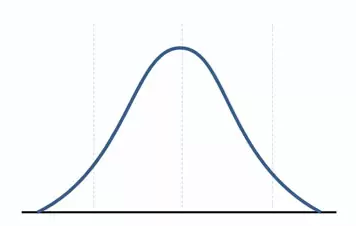
\includegraphics{gaussian.png}
\end{center}

\begin{itemize}
    \item amount of precipitation
    \item heights/weights of large populations
    \item measurement errors
    \item grades in courses
\end{itemize}

\begin{defbox}
    A normal random variable $ X $ with parameters $ \mu $ and $ \sigma^2 $ has pdf
    \[ f(x)=\frac{1}{\sqrt{2\pi}\sigma}e^{-(x-\mu)^2/(2\sigma^2)}\]
    for $ x\in\mathbb{R} $
\end{defbox}
\begin{itemize}
    \item symmetric around $ \mu $
    \item both tails go to zero quickly
    \item $\frac{1}{\sqrt{2\pi}\sigma}$ makes it integrate to 1.
\end{itemize}

\begin{center}
    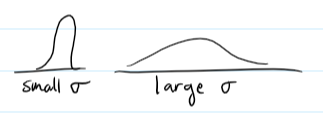
\includegraphics{sigma.png}
\end{center}
We can show that $ E[X]=\mu $ and $ Var(X)=\sigma^2 $

\subsection{Empirical rule}
\begin{center}
    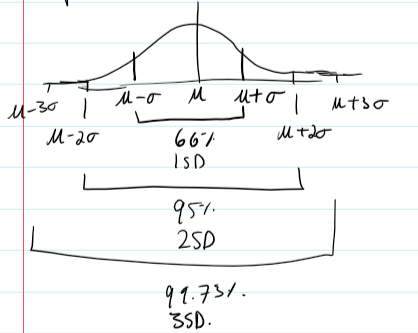
\includegraphics{emp.png}
\end{center}

\textsc{Find $ f(x) $}
\[ F(x)=\int\limits_{-\infty}^{x} \frac{1}{\sqrt{2\pi}\sigma}e^{-(u-\mu)^2/(2\sigma^2)} d{u} \]
\begin{itemize}
    \item not analytically integrable
    \item look it up or numerically evaluate
\end{itemize}
Standard Normal random variable (special case with $ \mu=0,\,\sigma^2=1 $)

$ Z \thicksim N(0,1) $
\[ f(z)=\frac{1}{\sqrt{2\pi}}e^{-z^2/2} \]
$ F(z) $ still has no closed form.
